\chapter{Filesystems}

\epigraph{\texttt{/home} is where another mount point should be if you are fault tolerant}{Bhuvy}

\section{What is a filesystem?}

You may have encountered the old unix adage, "everything is a file". In most UNIX systems, files operations provide an interface to abstract many different operations. Network sockets, hardware devices and even data on disk are all represented by a file-like object. A file-like object must follow certain conventions:

\begin{enumerate}
  \item It must present it self to the filesystem
  \item It must support common filesystem operations, such as \keyword{open}, \keyword{read}, \keyword{write}
\end{enumerate}

A filesystem is an implementation of the file interface. In this chapter, we will be exploring the various callbacks a filesystem provides and some typical functionality or implementation details associated with this. In this class, we will mostly talk about filesystems that serve to allow users to access data on disk. These filesystems are integral to modern computers. Filesystems not only deal with storing local files, they handle special devices that allow for safe communication between the kernel and user space. Filesystems also deal with failures, scalability, indexing, encryption, compression and performance. Filesystems handle the abstraction between a file which contains data and how exactly that data is stored on disk, partitioned, and protected.

Although filesystems are usually thought of as a kind of tree, most filesystems are usually a directed graph, a model we will explore in depth later in this chapter. Before we dive into the details of a filesystem, let's take a look at some examples.

\begin{enumerate}

  \item \keyword{ext4} Usually mounted at /, this is the filesystem that usually provides disk access as you're used to.
  \item \keyword{procfs} Usually mounted at /proc, provides information and control over processes.
  \item \keyword{sysfs} Usually mounted at /sys, a more modern version of /proc that also allows control over various other hardware such as network sockets.
  \item \keyword{tmpfs} Mounted at /tmp in some systems, an in-memory filesystem to hold temporary files.
  \item \keyword{sshfs} A filesystem that syncs files across the ssh protocol.

\end{enumerate}

To clarify, a mount point is simply a mapping of a directory to a filesystem represented in the kernel. What this means is that to resolve which filesystem a structure a call must resolve to. Meaning that \keyword{/root} is resolved by the \keyword{ext4} filesystem in our case, but \keyword{/proc/2} is resolved by the \keyword{procfs} system even though it contains \keyword{/} as a subsystem.

As you may have noticed, some of these filesystems provide an interface to things that aren't a "file" as you might colloquially refer to them. Filesystems such as \keyword{procfs} are usually referred to as \emph{virtual} filesystems, since they don't provide data access in the same sense as a traditional filesystem would. Technically, all filesystems in the kernel are represented by virtual filesystem, but in our class we will differentiate \emph{virtual} filesystems as filesystems that actually don't store anything on a hard disk.

\subsection{The File API}

A filesystem must provide callback functions to a variety of actions. Some of them as listed below:

\begin{itemize}
  \item \keyword{open} Opens a file for IO
  \item \keyword{read} Read contents of a file
  \item \keyword{write} Write to a file
  \item \keyword{close} Close a file and free associated resources
  \item \keyword{chmod} Modify permissions of a file
  \item \keyword{ioctl} Interact with device parameters of character devices such as terminals
\end{itemize}

Not every filesystem supports all the possible callback functions. For example many filesystems do not implement \keyword{ioctl} or \keyword{link}. In this chapter, we will not be examining each filesystem callback. If you would like to learn more about this interface, try looking at the documentation for FUSE, the source code for glibc or the linux man pages.

\section{Storing data on disk}

In order to understand how a filesystem interacts with data on disk, there are three key terms we will be using.
\begin{enumerate}
  \item \keyword{disk block} A disk block is a portion of the disk that is reserved for storing the contents of a file or a directory.
  \item \keyword{inode} An inode \emph{is} a file or directory. This means that an inode contains metadata about the file as well as pointers to disk blocks so that the file can actually be written to or read from.
  \item \keyword{superblock} A superblock contains metadata about the inodes and disk blocks. An example superblock can store how full each disk block is, which inodes are being used etc. Modern filesystems may actually contain multiple superblocks and a sort-of super-super block that keeps track of which sectors are governed by which superblocks. This tends to help with fragmentation.
\end{enumerate}

These structures all are presented in the diagram below.

\begin{figure}[htbp]
\centering
\includegraphics[width=.8\textwidth]{filesystems/images/disk.gif}
\caption{Disk block diagram}
\end{figure}

It may seem overwhelming, but by the end of this chapter, we will be able to make sense of every part of the filesystem.

In order to reason about data on some form of storage (spinning disks, solid state drives, magnetic tape, etc.), it is common practice to first consider the medium of storage as a collection of \emph{blocks}. A block can be thought of as a contiguous region on disk, and while it's size is sometimes determined by some property of the underlying hardware, it is more frequently determined based off of the size of a page of memory for a given system, so that data from the disk can be cached in memory for faster access - a very important feature of many filesystems.

Usually, a filesystem has a special block denoted as a \emph{superblock} which stores metadata about the filesystem such as a journal (which logs changes to the filesystem), a table of inodes and where the first inode is stored on disk, etc. The important thing about a superblock is that it is in a known location on disk.

The inode is the most important structure for our filesystem as it represents a file. Before we explore it in depth, let's list out the key information we need to have a usable file:

\begin{itemize}
\tightlist
  \item Name
  \item File size
  \item Time created, last modified, last accessed
  \item Permissions
  \item Filepath
  \item Checksum
  \item File data
\end{itemize}

\subsection{File Contents}

\begin{figure}[htbp]
\centering
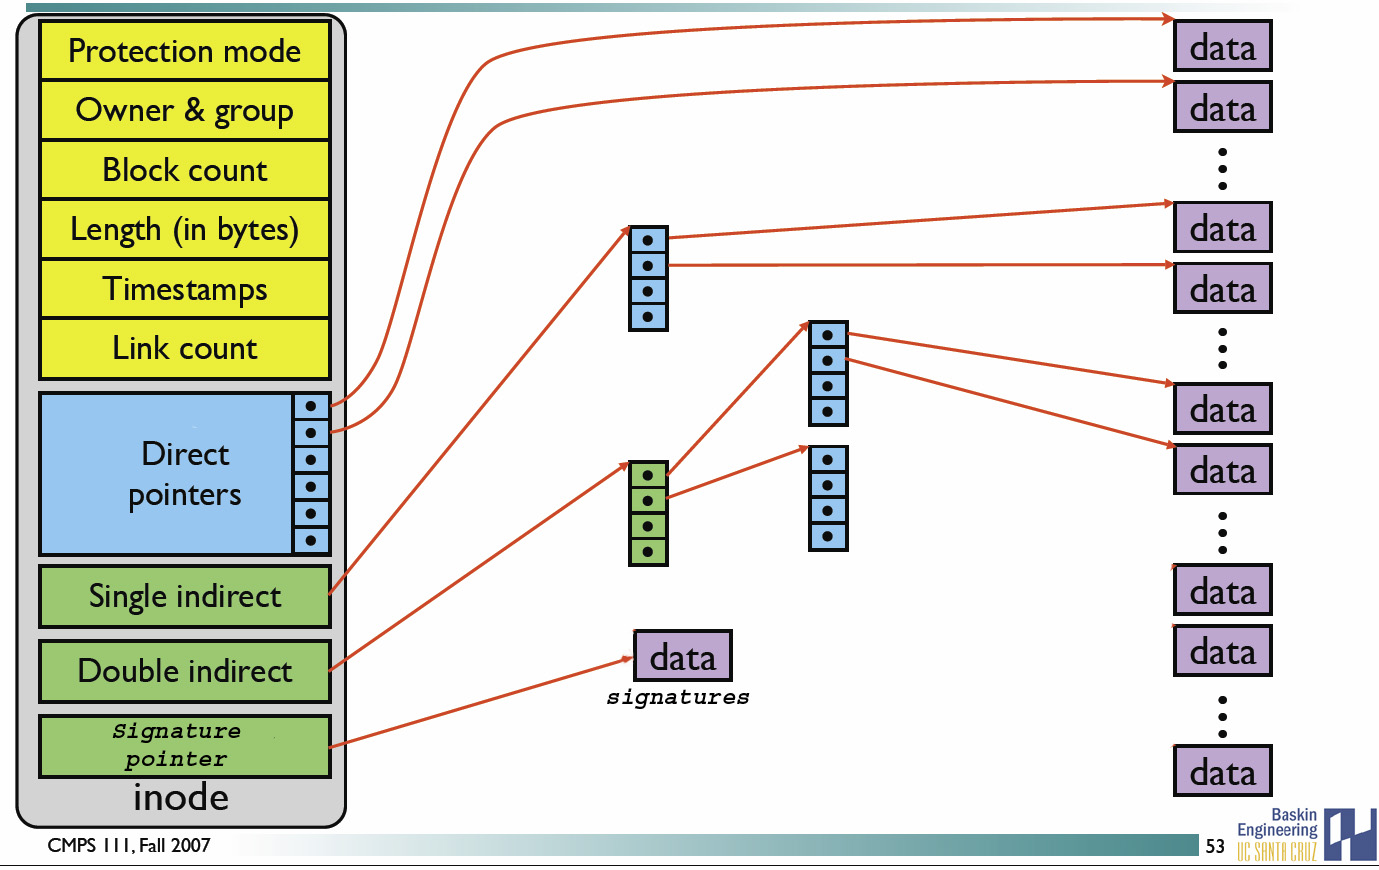
\includegraphics[width=.8\textwidth]{filesystems/images/inode_with_signatures.jpg}
\caption{Inode with contents}
\end{figure}

From \href{http://en.wikipedia.org/wiki/Inode}{Wikipedia}:

\begin{quote}
\emph{In a Unix-style file system, an index node, informally referred to as an inode, is a data structure used to represent a filesystem object, which can be one of various things including a file or a directory. Each inode stores the attributes and disk block location(s) of the filesystem object's data. Filesystem object attributes may include manipulation metadata (e.g.~change, access, modify time), as well as owner and permission data (e.g.~group-id, user-id, permissions).}
\end{quote}

Typically, the superblock stores an array of inodes, each of which stores direct, and potentially several kinds of indirect pointers to disk blocks. Since inodes are stored in the superblock, most filesystems have a limit on how many inodes can exist. Since each inode corresponds to a file, this is also a limit on how many files that filesystem can have. Trying to overcome this problem by storing inodes in some other location greatly increases the complexity of the filesystem. Trying to reallocate space for the inode table is also infeasible since every byte following the end of the inode array would have to be shifted, a highly expensive operation. This isn't to say there aren't any solutions at all, although typically there is no need to increase the number of inodes since the number of inodes is usually sufficiently high.

Big idea: Forget names of files: The `inode' is the file.

It is common to think of the file name as the `actual' file. It's not! Instead consider the inode as the file. The inode holds the meta-information (last accessed, ownership, size) and points to the disk blocks used to hold the file contents. However, the inode does not usually store a filename. Filenames are usually only stored in directories. (see below)

For example, to read the first few bytes of the file, follow the first direct block pointer to the first direct block and read the first few bytes. Writing follows the same process. If you want to read the entire file, keep reading direct blocks until you've read a number of bytes equal to the size of the file. If the total size of the file is less than that of the number of direct blocks multiplied by the size of a block, then unused block pointers will be undefined. Similarly, if the size of a file is not a multiple of the size of a block, data past the end of the last byte in the last block will be garbage.

What if a file is bigger than the maximum space addressable by it's direct blocks?

\begin{quote}
``All problems in computer science can be solved by another level of indirection.'' - David Wheeler
\end{quote}

Except the problem of too many layers of indirection.

To solve this problem, we introduce the indirect blocks. An indirect block is a block that store pointers to more data blocks. Similarly a double indirect block stores pointers to indirect blocks and the concept can be generalized to arbitrary levels of indirection. This is a very important concept, since as inodes are stored in the superblock, or some other structure in a well known location with a constant amount of space, indirection allows exponential increases in the amount of space an inode can keep track of.

As a worked example, suppose we divide the disk into 4KB blocks and we want to address up to 2\^{}32 blocks. The maximum disk size is 4KB *2\^{}32 = 16TB (remember 2\^{}10 = 1024). A disk block can store 4KB / 4B (each pointer needs to be 32 bits) = 1024 pointers. Each pointer refers to a 4KB disk block - so you can refer up to 1024*4KB = 4MB of data. For the same disk configuration, a double indirect block stores 1024 pointers to 1024 indirection tables. Thus a double-indirect block can refer up to 1024 * 4MB = 4GB of data. Similarly, a triple indirect block can refer up to 4TB of data. Naturally though, this is three times as slow.

\subsection{Directory Implementation}

A directory is just a mapping of names to inode numbers. It's typically just a normal file, but with some special bits set in its inode and a very specific structure for its contents. POSIX provides a small set of functions to read the filename and inode number for each entry, which we will talk about in depth later in this chapter.

Let's think about what it looks like in the actual file system. Theoretically, directories are just like actual files. The disk blocks will contain \emph{directory entries} or \emph{dirents}. What that means is that our disk block can look like this

\begin{verbatim}
| inode_num | name   | | ----------- | ------ |
| 2043567   | hi.txt | | ... |
\end{verbatim}

Each directory entry could either be a fixed size, or a variable c-string. It depends on how the particular filesystem implements it at the lower level. To see a mapping of filenames to inode numbers on a POSIX system, from a shell, use \keyword{ls} with the \keyword{-i} option

\begin{verbatim}
# ls -i
12983989 dirlist.c      12984068 sandwich.c
\end{verbatim}

\subsection{Unix Directory Conventions}

In standard unix file systems the following entries are specially added on requests to read a directory.

\begin{enumerate}
  \item \keyword{.} represents the current directory
  \item \keyword{..} represents the parent directory
  \item \keyword{~~} is the name of the home directory usually
\end{enumerate}

Note that \keyword{...} is NOT a valid representation of any directory (this not the grandparent directory). It \emph{could} however be the name of a file on disk. Though confusingly, \keyword{zsh} provides this as a handy shortcut to the grandparent directory should it exist.

Additional facts about name-related conventions:
\begin{enumerate}
  \item Files that start with '.' on disk are conventionally considered 'hidden' and will not be listed by programs like \keyword{ls} without additional flags (\keyword{-a}). This is not a feature of the filesystem and programs may choose to ignore this.
  \item Some files may also start with a null byte. These are usually \emph{abstract unix sockets} and are used to prevent cluttering up the filesystem since they will be effectively hidden by any program not expecting them. They will, however, be listed by tools that detail information about sockets, so this is not a feature providing security.
\end{enumerate}

\subsection{How do I list the contents of a directory?}

While interacting with a file in C is done by using \keyword{open} to open the file and then \keyword{read} or \keyword{write} to interact with the file before calling \keyword{close} to release resources, directories have special calls such as, \keyword{opendir}, \keyword{closedir} and \keyword{readdir}. There is no function \keyword{writedir} since typically that implies creating a file or link.

To explore these functions, let's write a program to search the contents of a directory for a particular file. (The code below has a bug, try to spot it!)

\begin{lstlisting}[language=C]
int exists(char *directory, char *name)  {
    struct dirent *dp;
    DIR *dirp = opendir(directory);
    while ((dp = readdir(dirp)) != NULL) {
        puts(dp->d_name);
        if (!strcmp(dp->d_name, name)) {
        return 1; /* Found */
        }
    }
    closedir(dirp);
    return 0; /* Not Found */
}
\end{lstlisting}

The above code has a subtle bug: It leaks resources! If a matching filename is found then `closedir' is never called as part of the early return. Any file descriptors opened, and any memory allocated, by opendir are never released. This means eventually the process will run out of resources and an \keyword{open} or \keyword{opendir} call will fail.

The fix is to ensure we free up resources in every possible code-path. In the above code this means calling \keyword{closedir} before \keyword{return 1}. Forgetting to release resources is a common C programming bug because there is no support in the C lanaguage to ensure resources are always released with all codepaths.


Note: after a call to fork(), either (XOR) the parent or the child can use readdir(), rewinddir() or seekdir(). If both the parent and the child use the above, behavior is undefined.

There are two main gotchas and one consideration: The \keyword{readdir} function returns ``.'' (current directory) and ``..'' (parent directory). If you are looking for sub-directories, you need to explicitly exclude these directories.

For many applications it's reasonable to check the current directory first before recursively searching sub-directories. This can be achieved by storing the results in a linked list, or resetting the directory struct to restart from the beginning.

The following code attempts to list all files in a directory recursively. As an exercise, try to identify the bugs it introduces.

\begin{lstlisting}[language=C]
void dirlist(char *path) {

  struct dirent *dp;
  DIR *dirp = opendir(path);
  while ((dp = readdir(dirp)) != NULL) {
     char newpath[strlen(path) + strlen(dp->d_name) + 1];
     sprintf(newpath,"%s/%s", newpath, dp->d_name);
     printf("%s\n", dp->d_name);
     dirlist(newpath);
  }
}

int main(int argc, char **argv) { dirlist(argv[1]); return 0; }
\end{lstlisting}

Did you find all 5 bugs?

\begin{lstlisting}[language=C]
// Check opendir result (perhaps user gave us a path that can not be opened as a directory
if (!dirp) { perror("Could not open directory"); return; }
// +2 as we need space for the / and the terminating 0
char newpath[strlen(path) + strlen(dp->d_name) + 2];
// Correct parameter
sprintf(newpath,"%s/%s", path, dp->d_name);
// Perform stat test (and verify) before recursing
if (0 == stat(newpath,&s) && S_ISDIR(s.st_mode)) dirlist(newpath)
// Resource leak: the directory file handle is not closed after the while loop
closedir(dirp);
\end{lstlisting}

One final note of caution: \keyword{readdir} is not thread-safe! Additionally \keyword{readdir\_r} is deprecated, so multi-threaded searches use \keyword{readdir} with external synchronization.

See the man page of readdir for more details.

\subsection{Linking}

Links are what force us to model a filesystem as a tree rather than a graph. While modelling the filesystem as a tree would imply that every inode has a unique parent directory, links allow inodes to present themselves as files in multiple places, potentially with different names, thus leading to an inode having multiple parents directories.

The first kind of link is a hard link. A hard link is simply an entry in a directory assigning some name to an inode number that already has a different name and mapping in either the same directory or a different one. If we already have a file on a file system we can create another link to the same inode using the `ln' command:

\begin{verbatim}
$ ln file1.txt blip.txt
\end{verbatim}

However blip.txt \emph{is} the same file; if I edit blip I'm editing the same file as `file1.txt!' We can prove this by showing that both file names refer to the same inode:

\begin{verbatim}
$ ls -i file1.txt blip.txt
134235 file1.txt
134235 blip.txt
\end{verbatim}

The equivalent C call is \keyword{link}

\begin{lstlisting}[language=C]
// Function Prototype
int link(const char *path1, const char *path2);

link("file1.txt", "blip.txt");
\end{lstlisting}

For simplicity the above examples made hard links inside the same directory. Hard links can be created anywhere inside the same filesystem.

The second kind of link is a soft link - or a symbolic link or a symlink. A symbolic link is different because it does not deal with inode numbers directly. Instead a symbolic link is a regular file with a special bit set and stores a path to another file. Quite simply, without the special bit, it is nothing more than a text file with a file path inside. Note that when people generally talk about a link without specifying hard or soft, they are referring to a hard link.

To create a symbolic link in the shell use \keyword{ln -s}. To read the contents of the link as just a file use \keyword{readlink}. These are both demonstrated below:

\begin{verbatim}
$ ln -s file1.txt file2.txt
$ ls -i file1.txt blip.txt
134235 file1.txt
134236 file2.txt
134235 blip.txt
$ cat file1.txt
file1!
$ cat file2.txt
file1!
$ cat blip.txt
file1!
$ echo edited file2 >> file2.txt # >> is bash syntax for append to file
$ cat file1.txt
file1!
edited file2
$ cat file2.txt
I'm file1!
edited file2
$ cat blip.txt
file1!
edited file2
$ readlink myfile.txt
file2.txt
\end{verbatim}

Note that \keyword{file2.txt} and \keyword{file1.txt} have different inode numbers, unlike the hard link, \keyword{blip.txt}.

There is a C library call to create symlinks which is similar to link:

\begin{lstlisting}[language=C]
symlink(const char *target, const char *symlink);
\end{lstlisting}

Some advantages of symbolic links are

\begin{itemize}
\tightlist
\item
  Can refer to files that don't exist yet
\item
  Unlike hard links, can refer to directories as well as regular files
\item
  Can refer to files (and directories) that exist outside of the current file system
\end{itemize}

However, symlinks have a key disadvantage, they as slower than regular files and directories. When the links contents are read, they must be interpreted as a new path to the target file, resulting in an additional call to open and read since the real file must be opened and read. Another disadvantage is that POSIX will not let you hard link directories whereas soft links are allowed. The \keyword{ln} command will only allow root to do this and only if you provide the \keyword{-d} option. However even root may not be able to perform this because most filesystems prevent it!

The integrity of the file system assumes the directory structure (excluding softlinks which we will talk about later) is a non-cyclic tree that is reachable from the root directory. It becomes expensive to enforce or verify this constraint if directory linking is allowed. Breaking these assumptions can cause file integrity tools to not be able to repair the file system. Recursive searches potentially never terminate and directories can have more than one parent but ``..'' can only refer to a single parent. All in all, a bad idea.

When you remove a file (using \keyword{rm} or \keyword{unlink}) you are removing an inode reference from a directory. However the inode may still be referenced from other directories. In order to determine if the contents of the file are still required, each inode keeps a reference count that is updated whenever a new link is created or destroyed. This count only tracks hard links, symlinks are allowed to refer to a non-existent file and thus, do not matter.

An example use of hard-links is to efficiently create multiple archives of a file system at different points in time. Once the archive area has a copy of a particular file, then future archives can re-use these archive files rather than creating a duplicate file. Apple's ``Time Machine'' software does this.

\subsection{Pathing}

Now that we have definitions talk about directories, we come across the concept of a path. A path is a sequence of directories that provide one with a "path" in the filesystem graph. However, there are some nuances. It is possible to have a path called \texttt{a/b/../c/./}. Since \keyword{..} and \keyword{.} are special entries in directories, this is a valid path that actually refers to \texttt{a/c}. Most filesystem functions will allow uncompressed paths to be passed in. The C library provides a function \keyword{realpath} to compress the path or get the realpath. To simplify by hand remember that \keyword{..} means `parent folder' and that \keyword{.} means `current folder'. Below is an example that illustrates the simplification of the \texttt{a/b/../c/.} by using \keyword{cd} in a shell to navigate a filesystem.

\begin{enumerate}
  \item \keyword{cd a} (in a)
  \item \keyword{cd b} (in a/b)
  \item \keyword{cd ..} (in a, because .. represents `parent folder')
  \item \keyword{cd c} (in a/c)
  \item \keyword{cd .} (in a/c, because . represents `current folder')
\end{enumerate}

Thus, this path can be simplified to \keyword{a/c}.

\subsection{Metadata}

How can we distinguish between a regular file and a directory? For that matter there's many other attributes that files also might contain. You may know that on most UNIX systems, unlike windows systems, a file's type is not determined by its extension. How does the system know what type the file is?

All of this information is stored within an inode. To access it, use the stat calls. For example, to find out when my `notes.txt' file was last accessed.

\begin{lstlisting}[language=C]
struct stat s;
stat("notes.txt", &s);
printf("Last accessed %s", ctime(&s.st_atime));
\end{lstlisting}

There are actually three versions of \keyword{stat};

\begin{lstlisting}[language=C]
int stat(const char *path, struct stat *buf);
int fstat(int fd, struct stat *buf);
int lstat(const char *path, struct stat *buf);
\end{lstlisting}

For example, you can use \keyword{fstat} to find out the meta-information about a file if you already have an file descriptor associated with that file

\begin{lstlisting}[language=C]
FILE *file = fopen("notes.txt", "r");
int fd = fileno(file); /* Just for fun - extract the file descriptor from a C FILE struct */
struct stat s;
fstat(fd, & s);
printf("Last accessed %s", ctime(&s.st_atime));
\end{lstlisting}

\keyword{lstat} is almost the same as \keyword{stat} but handles symbolic links differently. From the \keyword{stat} man page:
\begin{quote}
lstat() is identical to stat(), except that if pathname is a symbolic link, then it returns information about the link itself, not the file that it refers to.
\end{quote}

The stat functions make use of \keyword{struct stat}. From the \keyword{stat} man page:

\begin{lstlisting}[language=C]
struct stat {
    dev_t     st_dev;         /* ID of device containing file */
    ino_t     st_ino;         /* Inode number */
    mode_t    st_mode;        /* File type and mode */
    nlink_t   st_nlink;       /* Number of hard links */
    uid_t     st_uid;         /* User ID of owner */
    gid_t     st_gid;         /* Group ID of owner */
    dev_t     st_rdev;        /* Device ID (if special file) */
    off_t     st_size;        /* Total size, in bytes */
    blksize_t st_blksize;     /* Block size for filesystem I/O */
    blkcnt_t  st_blocks;      /* Number of 512B blocks allocated */
    struct timespec st_atim;  /* Time of last access */
    struct timespec st_mtim;  /* Time of last modification */
    struct timespec st_ctim;  /* Time of last status change */
};
\end{lstlisting}

The \keyword{st\_mode} field can be used to distinguish between regular files and directories. To accomplish this, you will also need the macros, \keyword{S\_ISDIR} and \keyword{S\_ISREG}.

\begin{lstlisting}[language=C]
   struct stat s;
   if (0 == stat(name, &s)) {
      printf("%s ", name);
      if (S_ISDIR( s.st_mode)) puts("is a directory");
      if (S_ISREG( s.st_mode)) puts("is a regular file");
   } else {
      perror("stat failed - are you sure I can read this file's meta data?");
   }
\end{lstlisting}

\section{Permissions and bits}

Permissions are a key part of the way UNIX systems provide security in a filesystem. You may have noticed that the \keyword{st\_mode} field in \keyword{struct stat} contains more than just the file type. It also contains the mode, a description detailing what a user can and can't do with a given file. There are usually three sets of permissions for any file. Permissions for the \emph{user}, the \emph{group} and \emph{other}. For each of the three categories we need to keep track of whether or not the user is allowed to read the file, write to the file, and execute the file. Since there are three categories and three permissions, permissions are usually represented as a 3-digit octal number. For each digit the least significant byte corresponds to read privileges, the middle one to write privileges and the final byte to execute privileges. They are always presented as \emph{User}, \emph{Group}, \emph{Other} (\emph{UGO}). Below are some common examples:

\begin{enumerate}

\item 755: \keyword{rwx r-x r-x}

user: \keyword{rwx}, group: \keyword{r-x}, others: \keyword{r-x}

User can read, write and execute. Group and others can only read and execute.

\item 644: \keyword{rw- r-- r--}

user: \keyword{rw-}, group: \keyword{r--}, others: \keyword{r--}

User can read and write. Group and others can only read.

\end{enumerate}

It is worth noting that the \keyword{rwx} bits for a directory have slightly different meaning. Write-access to a directory will allow you to create or delete new files or directories inside (you can think about this as just having write access to the dirent mappings). Read-access to a directory will allow you to list a directory's contents (this is just read access to the dirent mapping). Execute will allow you to enter the directory and access it. Without the execute bit it is not possible to create or remove files or directories since you cannot access them. You can, however, list the contents of the directory.

There are several command line utilities for interacting with a file's mode. \keyword{mknod} changes the type of the file. \keyword{chmod} takes a number and a file and changes the permission bits. However, before we can discuss chmod in detail, we must also understand the user id (\keyword{uid}) and group id (\keyword{gid}) as well.

\subsection{User id/Group id}
Every user in a UNIX system has a user id. This is a unique number that can identify a user. Similarly, users can be added to collections called groups, and every group also has a uniquely identifying number. Groups have a variety of uses on UNIX systems. They can be assigned capabilities - a way of describing the level of control a user has over a system. For example, a group you may have run into is the \keyword{sudoers} group, a set of trusted users who are allowed to use the command \keyword{sudo} to temporarily gain higher privileges. (We'll talk more about how \keyword{sudo} works in this chapter). Every file, upon creation, an owner, the creator of the file. This owner's user id (\keyword{uid}) can be found inside the \keyword{st\_mode} file of a \keyword{struct stat} with a call to \keyword{stat}. Similarly the group id (\keyword{gid}) is set as well.

Every process can determine it's \keyword{uid} and \keyword{gid} with \keyword{getuid} and \keyword{getgid}. When a processes tries to open a file with a specific mode, it's \keyword{uid} and \keyword{gid} are compared with the \keyword{uid} and \keyword{gid} of the file. If the \keyword{uid}s match, then the process's request to open the file will be compared with the bits on the user field of the file's permissions. Similarly, if the \keyword{gid}s match, then the process's request will be compared with the group field of the permissions. Finally, if none of the ids match, then the other field will apply.

\subsection{Reading/Changing file permissions}

Before we discuss how to change permission bits, we should be able to read them. In C, the \keyword{stat} family of library calls can be used. To read permission bits from the command line, use `ls -l'. Note that the permissions will outputed in the format `drwxrwxrwx'. The first character indicates the type of file type. Possible values for the first character:

\begin{enumerate}
\item (-) regular file
\item (d) directory
\item (c) character device file
\item (l) symbolic link
\item (p) pipe
\item (b) block device
\item (s) socket
\end{enumerate}

Alternatively, use the program \keyword{stat} which presents all the information that one could retrieve from the \keyword{stat} library call.

To change the permission bits, there is a system call, \keyword{int chmod(const char *path, mode\_t mode);}. In order to simplify our examples, we will be using the command line utility of the same name \keyword{chmod} (short of ``change mode''). There are two common ways to use \keyword{chmod} ; either with an octal value or with a symbolic string:

\begin{verbatim}
$ chmod 644 file1
$ chmod 755 file2
$ chmod 700 file3
$ chmod ugo-w file4
$ chmod o-rx file4
\end{verbatim}

The base-8 (`octal') digits describe the permissions for each role: The user who owns the file, the group and everyone else. The octal number is the sum of three values given to the three types of permission: read(4), write(2), execute(1)

Example: chmod 755 myfile

\begin{enumerate}
\item r + w + x = digit * user has 4+2+1, full permission
\item group has 4+0+1, read and execute permission
\item all users have 4+0+1, read and execute permission
\end{enumerate}

\subsection{Understanding the `umask'}

The umask \emph{subtracts} (reduces) permission bits from \keyword{777} and is used when new files and new directories are created by open, mkdir etc. By default the umask is set to \keyword{022} (octal), which means that group and other privileges will not include the writable bit . Each process (including the shell) has a current umask value. When forking, the child inherits the parent's umask value.

For example, by setting the umask to \keyword{077} in the shell, ensures that future file and directory creation will only be accessible to the current user,

\begin{verbatim}
$ umask 077
$ mkdir secretdir
\end{verbatim}

As a code example, suppose a new file is created with \keyword{open()} and mode bits \keyword{666} (write and read bits for user,group and other):

\begin{lstlisting}[language=C]
open("myfile", O_CREAT, S_IRUSR | S_IWUSR | S_IRGRP | S_IWGRP | S_IROTH | S_IWOTH);
\end{lstlisting}

If umask is octal \keyword{022}, then the permissions of the created file will be \keyword{0666} \& \textasciitilde{}\keyword{022} ie.

\begin{lstlisting}[language=C]
S_IRUSR | S_IWUSR | S_IRGRP | S_IROTH
\end{lstlisting}

\subsection{The `setuid' bit}

You may have noticed an additional bit that files with execute permission may have set. This bit is the \keyword{setuid} bit. It indicated that when run, the program with set the uid of the user to that of the owner of the file. Similar, there is a \keyword{setgid} bit which sets the gid of the executor to the gid of the owner. The canonical example of a program with \keyword{setuid} set is \keyword{sudo}.

\keyword{sudo} is usually a program that is owned by the root user - a user that has all capabilities. By using \keyword{sudo} an otherwise unprivileged user can gain access to most parts of the system. This is useful for running programs that may require elevated privileges, such as using \keyword{chown} to change ownership of a file, or to use \keyword{mount} to mount or unmount filesystems (an action we will discuss later in this chapter). Here are some examples:

\begin{verbatim}
$ sudo mount /dev/sda2 /stuff/mydisk
$ sudo adduser fred
$ ls -l /usr/bin/sudo
-r-s--x--x  1 root  wheel  327920 Oct 24 09:04 /usr/bin/sudo
\end{verbatim}

\subsubsection{Effective uid/gid}

When executing a process with the setuid bit, it is still possible to determine a user's original uid with \keyword{getuid}. The real action of the \keyword{setuid} bit is to set the effective userid (\keyword{euid}) which can be determined with \keyword{geteuid}. The actions of \keyword{getuid} and \keyword{geteuid} are described below.

\begin{itemize}
\tightlist
\item
  \keyword{getuid} returns the real user id (zero if logged in as root)
\item
  \keyword{geteuid} returns the effective userid (zero if acting as root, e.g.~due to the setuid flag set on a program)
\end{itemize}

These functions can allow one to write a program that can only be run by a privileged user by checking \keyword{geteuid} or go a step further and ensure that the only user who can run the code is root by using \keyword{getuid}.

\subsection{The `sticky' bit}

Sticky bits as we use them today do not serve the same purpose as their initial introduction. Sticky bits were a bit that could be set on an executable file that would allow a program's text segment to remain in swap even after the end of the program's execution. This made subsequent executions of the same program faster. Today, this behavior is no longer supported and the sticky bit only holds meaning when set on a directory,

When a directory's sticky bit is set only the file's owner, the directory's owner, and the root user can rename or delete the file. This is useful when multiple users have write access to a common directory. A common use of the sticky bit is for the shared and writable \keyword{/tmp} directory.

To set the sticky bit, use \keyword{chmod +t}.

\begin{verbatim}
aneesh$ mkdir sticky
aneesh$ chmod +t sticky
aneesh$ ls -l
drwxr-xr-x  7 aneesh aneesh    4096 Nov  1 14:19 .
drwxr-xr-x 53 aneesh aneesh    4096 Nov  1 14:19 ..
drwxr-xr-t  2 aneesh aneesh    4096 Nov  1 14:19 sticky
aneesh$ su newuser
newuser$ rm -rf sticky
rm: cannot remove 'sticky': Permission denied
newuser$ exit
aneesh$ rm -rf sticky
aneesh$ ls -l
drwxr-xr-x  7 aneesh aneesh    4096 Nov  1 14:19 .
drwxr-xr-x 53 aneesh aneesh    4096 Nov  1 14:19 ..
\end{verbatim}

Note that in the example above, the username is prepended to the prompt, and the command \keyword{su} is used to switch users.

\section{Virtual filesystems and other filesystems}

POSIX systems, such as Linux and Mac OSX (which is based on BSD) include several virtual filesystems that are mounted (available) as part of the file-system. Files inside these virtual filesystems do not exist on the disk; they are generated dynamically by the kernel when a process requests a directory listing. Linux provides 3 main virtual filesystems

\begin{verbatim}
/dev  - A list of physical and virtual devices (for example network card, cdrom, random number generator)
/proc - A list of resources used by each process and (by tradition) set of system information
/sys - An organized list of internal kernel entities
\end{verbatim}

For example if I want a continuous stream of 0s, I can \keyword{cat /dev/zero}.

Another example is the file \keyword{/dev/null} - a great place to store bits that you never need to read! Bytes sent to \keyword{/dev/null/} are never stored - they are simply discarded. A common use of \keyword{/dev/null} is to discard standard output. For example,

\begin{verbatim}
$ ls . >/dev/null
\end{verbatim}

\subsection{Managing files and filesystems}

Given the multitude of operations that are available to you from the filesystem, let's explore some tools and techniques that can be used to manage files and filesystems.

One example is creating a secure directory. Suppose you created your own directory in /tmp and then set the permissions so that only you can use the directory (see below). Is this secure?

\begin{verbatim}
$ mkdir /tmp/mystuff
$ chmod 700 /tmp/mystuff
\end{verbatim}

There is a window of opportunity between when the directory is created and when it's permissions are changed. This leads to several vulnerabilities that are based on a race condition.

Another user replaces \keyword{mystuff} with a hard link to an existing file or directory owned by the second user, then they would be able to read and control the contents of the \keyword{mystuff} directory. Oh no - our secrets are no longer secret!

However in this specific example the \keyword{/tmp} directory has the sticky bit set, so other users may not delete the \keyword{mystuff} directory, and the simple attack scenario described above is impossible. This does not mean that creating the directory and then later making the directory private is secure! A better version is to atomically create the directory with the correct permissions from its inception -

\begin{verbatim}
$ mkdir -m 700 /tmp/mystuff
\end{verbatim}

\subsection{Obtaining random data}

\keyword{/dev/random} is a file which contains number generator where the entropy is determined from environmental noise. Random will block/wait until enough entropy is collected from the environment.

\keyword{/dev/urandom} is like random, but differs in the fact that it allows for repetition (lower entropy threshold), thus wont block.


\subsection{Copying Files}

Use the versatile \keyword{dd} command. For example, the following command copies 1 MB of data from the file \keyword{/dev/urandom} to the file \keyword{/dev/null}. The data is copied as 1024 blocks of blocksize 1024 bytes.

\begin{verbatim}
$ dd if=/dev/urandom of=/dev/null bs=1k count=1024
\end{verbatim}

Both the input and output files in the example above are virtual - they don't exist on a disk. This means the speed of the transfer is unaffected by hardware power.

\keyword{dd} is also commonly used to make a copy of a disk or an entire filesystem to create images that can either be burned on to other disks or to distribute data to other users.

\subsection{Updating Modification Time}\label{what-happens-when-i-touch-a-file}

The \keyword{touch} executable creates file if it does not exist and also updates the file's last modified time to be the current time. For example, we can make a new private file with the current time:

\begin{verbatim}
$ umask 077       # all future new files will maskout all r,w,x bits for group and other access
$ touch file123   # create a file if it does not exist, and update its modified time
$ stat file123
  File: `file123'
  Size: 0           Blocks: 0          IO Block: 65536  regular empty file
Device: 21h/33d Inode: 226148      Links: 1
Access: (0600/-rw-------)  Uid: (395606/ angrave)   Gid: (61019/     ews)
Access: 2014-11-12 13:42:06.000000000 -0600
Modify: 2014-11-12 13:42:06.001787000 -0600
Change: 2014-11-12 13:42:06.001787000 -0600
\end{verbatim}

An example use of touch is to force make to recompile a file that is unchanged after modifying the compiler options inside the makefile. Remember that make is `lazy' - it will compare the modified time of the source file with the corresponding output file to see if the file needs to be recompiled

\begin{verbatim}
$ touch myprogram.c   # force my source file to be recompiled
$ make
\end{verbatim}

\subsection{Managing Filesystems}

To manage filesystems on your machine, use \keyword{mount}. Using mount without any options generates a list (one filesystem per line) of mounted filesystems including networked, virtual and local (spinning disk / SSD-based) filesystems. Here is a typical output of mount

\begin{verbatim}
$ mount
/dev/mapper/cs241--server_sys-root on / type ext4 (rw)
proc on /proc type proc (rw)
sysfs on /sys type sysfs (rw)
devpts on /dev/pts type devpts (rw,gid=5,mode=620)
tmpfs on /dev/shm type tmpfs (rw,rootcontext="system_u:object_r:tmpfs_t:s0")
/dev/sda1 on /boot type ext3 (rw)
/dev/mapper/cs241--server_sys-srv on /srv type ext4 (rw)
/dev/mapper/cs241--server_sys-tmp on /tmp type ext4 (rw)
/dev/mapper/cs241--server_sys-var on /var type ext4 (rw)rw,bind)
/srv/software/Mathematica-8.0 on /software/Mathematica-8.0 type none (rw,bind)
engr-ews-homes.engr.illinois.edu:/fs1-homes/angrave/linux on /home/angrave type nfs (rw,soft,intr,tcp,noacl,acregmin=30,vers=3,sec=sys,sloppy,addr=128.174.252.102)
\end{verbatim}

Notice that each line includes the filesystem type source of the filesystem and mount point. To reduce this output we can pipe it into \keyword{grep} and only see lines that match a regular expression.

\begin{verbatim}
>mount | grep proc  # only see lines that contain 'proc'
proc on /proc type proc (rw)
none on /proc/sys/fs/binfmt_misc type binfmt_misc (rw)
\end{verbatim}

\subsubsection{Filesystem Mounting}\label{how-do-i-mount-a-disk-image}

Suppose you had downloaded a bootable linux disk image from the \href{http://cosmos.cites.illinois.edu/pub/archlinux/iso/2015.04.01/archlinux-2015.04.01-dual.iso}{URL}

\begin{verbatim}
wget $URL
\end{verbatim}

Before putting the filesystem on a CD, we can mount the file as a filesystem and explore its contents. Note, mount requires root access, so let's run it using sudo

\begin{verbatim}
$ mkdir arch
$ sudo mount -o loop archlinux-2015.04.01-dual.iso ./arch
$ cd arch
\end{verbatim}

Before the mount command, the arch directory is new and obviously empty. After mounting, the contents of \keyword{arch/} will be drawn from the files and directories stored in the filesystem stored inside the \keyword{archlinux-2014.11.01-dual.iso} file. The \keyword{loop} option is required because we want to mount a regular file not a block device such as a physical disk.

The loop option wraps the original file as a block device - in this example we will find out below that the file system is provided under \keyword{/dev/loop0} : We can check the filesystem type and mount options by running the mount command without any parameters. We will pipe the output into \keyword{grep} so that we only see the relevant output line(s) that contain `arch'

\begin{verbatim}
$ mount | grep arch
/home/demo/archlinux-2014.11.01-dual.iso on /home/demo/arch type iso9660 (rw,loop=/dev/loop0)
\end{verbatim}

The iso9660 filesystem is a read-only filesystem originally designed for optical storage media (i.e.~CDRoms). Attempting to change the contents of the filesystem will fail

\begin{verbatim}
$ touch arch/nocando
touch: cannot touch `/home/demo/arch/nocando': Read-only file system
\end{verbatim}

\section{Memory Mapped IO}

While we traditionally think of reading and writing from a file as operation that happen by using the \keyword{read} and \keyword{write} calls, there is an alternative, mapping a file into memory using \keyword{mmap}. \keyword{mmap} can also be used for IPC, and you can see more about \keyword{mmap} as a system call that enables shared memory in the IPC chapter. In this chapter, we'll briefly explore \keyword{mmap} as a filesystem operation.

\keyword{mmap} takes a file and maps its contents into memory. This allows a user to treat the entire file as a buffer in memory for easier semantics while programming, and to avoid having to read a file as discrete chunks explicitly.

Not all filesystems support using \keyword{mmap} for IO, but amongst those that do, not all have the same behavior. Some will simply implement \keyword{mmap} as a wrapper around \keyword{read} and \keyword{write}. Others will add additional optimizations by taking advantage of the kernel's page cache. Of course, such optimization can be used in the implementation of \keyword{read} and \keyword{write} as well, so often using \keyword{mmap} does not impact performance.

\keyword{mmap} is used to perform some operations such as loading libraries and processes into memory. If many programs only need read-access to the same file (e.g. \keyword{/bin/bash}, the C library) then the same physical memory can be shared between multiple processes.

The process to map a file into memory is simple:

\begin{enumerate}
\item \keyword{mmap} requires a file descriptor, so we need to \keyword{open} the file first
\item We seek to our desired size and write one byte to ensure that the file is sufficient length
\item When finished call munmap to unmap the file from memory.
\end{enumerate}

Here is a quick example.

\begin{lstlisting}[language=C]
#include <stdio.h>
#include <stdlib.h>
#include <sys/types.h>
#include <sys/stat.h>
#include <sys/mman.h>
#include <fcntl.h>
#include <unistd.h>
#include <errno.h>
#include <string.h>


int fail(char *filename, int linenumber) {
  fprintf(stderr, "%s:%d %s\n", filename, linenumber, strerror(errno));
  exit(1);
  return 0; /*Make compiler happy */
}
#define QUIT fail(__FILE__, __LINE__ )

int main() {
  // We want a file big enough to hold 10 integers
  int size = sizeof(int) * 10;

  int fd = open("data", O_RDWR | O_CREAT | O_TRUNC, 0600); //6 = read+write for me!

  lseek(fd, size, SEEK_SET);
  write(fd, "A", 1);

  void *addr = mmap(0, size, PROT_READ | PROT_WRITE, MAP_SHARED, fd, 0);
  printf("Mapped at %p\n", addr);
  if (addr == (void*) -1 ) QUIT;

  int *array = addr;
  array[0] = 0x12345678;
  array[1] = 0xdeadc0de;

  munmap(addr,size);
  return 0;

}
\end{lstlisting}

The careful reader may notice that our integers were written in least-significant-byte format (because that is the endianness of the CPU) and that we allocated a file that is one byte too many! The \keyword{PROT\_READ | PROT\_WRITE} options specify the virtual memory protection. The option \keyword{PROT\_EXEC} (not used here) can be set to allow CPU execution of instructions in memory (e.g.~this would be useful if you mapped an executable or library).

\section{Reliable Single Disk Filesystems}

Most filesystems cache significant amounts of disk data in physical memory. Linux, in this respect, is particularly extreme: All unused memory is used as a giant disk cache. The disk cache can have significant impact on overall system performance because disk I/O is slow. This is especially true for random access requests on spinning disks where the disk read-write latency is dominated by the seek time required to move the read-write disk head to the correct position.

For efficiency, the kernel caches recently used disk blocks. For writing, we have to choose a trade-off between performance and reliability: Disk writes can also be cached (``Write-back cache'') where modified disk blocks are stored in memory until evicted. Alternatively a `write-through cache' policy can be employed where disk writes are sent immediately to the disk. The latter is safer (as filesystem modifications are quickly stored to persistent media) but slower than a write-back cache; If writes are cached then they can be delayed and efficiently scheduled based on the physical position of each disk block. Note this is a simplified description because solid state drives (SSDs) can be used as a secondary write-back cache.

Both solid state disks (SSD) and spinning disks have improved performance when reading or writing sequential data. Thus operating system can often use a read-ahead strategy to amortize the read-request costs (e.g.~time cost for a spinning disk) and request several contiguous disk blocks per request. By issuing an I/O request for the next disk block before the user application requires the next disk block, the apparent disk I/O latency can be reduced.

If your data is important and needs to be force written to disk, call \keyword{sync} to request that a filesystem changes be written (flushed) to disk. However, not all operating systems honor this request and even if the data is evicted from the kernel buffers the disk firmware use an internal on-disk cache or may not yet have finished changing the physical media. Note you can also request that all changes associated with a particular file descriptor are flushed to disk using \keyword{fsync(int fd)}

If your operating system fails in the middle of an operation, most modern file systems do something called \textbf{journalling} that work around this. What the file system does is before it completes a potentially expensive operation, is that it writes what it is going to do down in a journal. In the case of a crash or failure, one can step through the journal and see which files are corrupt and fix them. This is a way to salvage hard disks in cases there is critical data and there is no apparent backup.

Even though it is unlikely for your computer, programming for data centers means that disks fail every few seconds. Disk failures are measured using ``Mean-Time-Failure''. For large arrays, the mean failure time can be surprisingly short. For example if the MTTF(single disk) = 30,000 hours, then the MTTF(1000 disks)= 30000/1000=30 hours or about a day and a half!

\subsection{RAID}\label{redundancy}

One way to protect against this is to store the data twice! This is the main principle of a ``RAID-1'' disk array. RAID is short for redundant array of inexpensive disks. By duplicating the writes to a disk with writes to another backup disk, there are exactly two copies of the data. If one disk fails, the other disk serves as the only copy until it can be re-cloned. Reading data is faster since data can be requested from either disk, but writes are potentially twice as slow because now two write commands need to be issued for every disk block write. Compared to using a single disk, the cost of storage per byte has doubled.

Another common RAID scheme is RAID-0, meaning that a file could be split up among two disks, but if any one of the disks fail then the files are irrecoverable. This has the benefit of halving write times because one part of the file could be writing to hard disk one and another part to hard disk two.

It is also common to combine these systems. If you have a lot of hard disks, consider RAID-10. This is where you have two systems of RAID-1, but the systems are hooked up in RAID-0 to each other. This means you would get roughly the same speed from the slowdowns but now any one disk can fail and you can recover that disk. If two disks from opposing raid partitions fail there is a chance that recover can happen though we don't could on it most of the time.

\subsection{Higher Level Raids}

RAID-3 uses parity codes instead of mirroring the data. For each N-bits written we will write one extra bit, the `Parity bit' that ensures the total number of 1s written is even. The parity bit is written to an additional disk. If any one disk (including the parity disk) is lost, then its contents can still be computed using the contents of the other disks.

\begin{figure}[htbp]
\centering
\includegraphics{filesystems/images/raid.gif}
\caption{Raid diagram}
\end{figure}

One disadvantage of RAID-3 is that whenever a disk block is written, the parity block will always be written too. This means that there is effectively a bottleneck in a separate disk. In practice, this is more likely to cause a failure because one disk is being used 100\% of the time and once that disk fails then the other disks are more prone to failure.

A single disk failure will not result in data loss (because there is sufficient data to rebuild the array from the remaining disks). Data-loss will occur when a two disks are unusable because there is no longer sufficient data to rebuild the array. We can calculate the probability of a two disk failure based on the repair time which includes not just the time to insert a new disk but the time required to rebuild the entire contents of the array.

\begin{verbatim}
MTTF = mean time to failure
MTTR = mean time to repair
N = number of original disks

p = MTTR / (MTTF-one-disk / (N-1))
\end{verbatim}

Using typical numbers (MTTR=1day, MTTF=1000days, N-1 = 9, p=0.009)

There is a 1\% chance that another drive will fail during the rebuild process (at that point you had better hope you still have an accessible backup of your original data. In practice the probability of a second failure during the repair process is likely higher because rebuilding the array is I/O-intensive (and on top of normal I/O request activity). This higher I/O load will also stress the disk array

RAID-5 is similar to RAID-3 except that the check block (parity information) is assigned to different disks for different blocks. The check-block is `rotated' through the disk array. RAID-5 provides better read and write performance than RAID-3 because there is no longer the bottleneck of the single parity disk. The one drawback is that you need more disks to have this setup and there are more complicated algorithms need to be used

\begin{figure}[htbp]
\centering
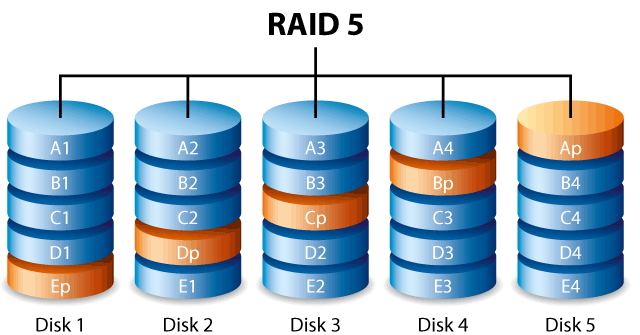
\includegraphics[width=.8\textwidth]{filesystems/images/raid_5.png}
\caption{Raid 5 striping}
\end{figure}

Failure is the common case. Google reports 2-10\% of disks fail per year Now multiply that by 60,000+ disks in a single warehouse\ldots{} Must survive failure of not just a disk, but a rack of servers or a whole data center

Solutions Simple redundancy (2 or 3 copies of each file) e.g., Google GFS (2001) More efficient redundancy (analogous to RAID 3++) e.g., \href{http://goo.gl/LwFIy}{Google Colossus filesystem} (\textasciitilde{}2010): customizable replication including Reed-Solomon codes with 1.5x redundancy

\section{Simple Filesystem Model}

Software developers need to implement filesystems all the time. Don't believe me? Take a look at Hadoop, GlusterFS,
Qumulo, etc. Filesystems are hot areas of research now because people have realized that the software models that we
devised don't take full advantage of our current hardware. Additionally, the hardware that we use for storing information
is getting better and better all the time. As such, you may end up designing a filesystem yourself someday. In this
section we will go over one of our fake filesystems that we talk about in class and ``walk through'' some examples of
how things work.

So what does our hypothetical filesystem look like? We will base it off of the \textt{minixfs}, a very simple filesystem
that happens to be the first filesystem that Linux ran on. Laid out sequentially on disk, we first have our superblock.
The superblock stores important metadata about the entire filesystem. Since we want to be able to read this block before
we know anything else about the data on disk, this needs to be in a well-known location so the very start of the disk is
a good choice. After the superblock, we'll keep a map of which inodes are being used. The n'th bit is set if the n'th
inode -- $0$ being the inode root -- is being used. Similarly, we store a map recording which datablocks are used.
Finally, we have an array of inodes followed by the rest of the disk - implicitly partitioned into datablocks. It's
important to note that there may not be any real distinction from one datablock to the next from the perspective of the
hardware components of the disk. Thinking about the disk as an array of datablocks is simply something we do so that we
have a way to describe where files live on disk.

Below, we have an example of how an inode that describes a file may look. Note that for the sake of simplicity, we have
drawn arrows mapping datablock numbers in the inode to their locations on disk, these aren't pointers so much as
indicies into an array.
\begin{figure}[htbp]
\centering
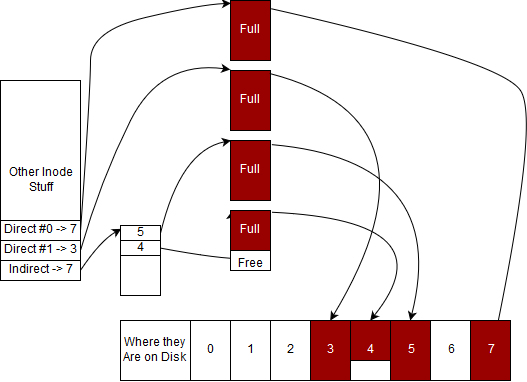
\includegraphics[width=.8\textwidth]{filesystems/images/sample_file.png}
\caption{Sample file filling up}
\end{figure}

We will assume that a data block is 4 KB.

Note that a file will fill up each of its data blocks completely before requesting an additional data block. We will
refer to this property as as the file being \textit{compact}. The file presented above is interesting since it uses all
of it's direct blocks, one of the entries for it's indirect block and partially uses another indirect block.

The following subsections will all refer to the file presented above.

\subsection{How big is our file?}
The size of a file is not something that we can compute by staring at it. We need additional information that is
typically stored in the inode. This is because the filesystem isn't aware of the actual contents of what is in a file.
That data is considered the user's. However, we can compute an upper bound by looking at how many blocks the file uses.

There are two full direct blocks, which together store $2*sizeof(data\_block)=2*4KB=8KB$.

There are two used blocks referenced by the indirect block, which can store up to $8KB$ as calculated above.

We can now add these values to get an upper bound on the file size of $16KB$.

What about a lower bound? We know that we must use the two direct blocks, one block referenced by the indirect block and at least 1 byte of a
second block referenced by the indirect block. With this information, we can work out the lower bound to be $2*4KB+4KB+1=12KB+1B$.

Note that our calculations so far have been to determine how much data the user is storing on disk. We have not
considered the \textit{overhead} of storing this data incurred while using this filesystem. You'll notice that we use an
indirect block to store the disk block numbers of blocks used beyond the two direct blocks. While doing our above
calculations, we did not take this block into account while computing the filesize. This would instead be counted as the
overhead of the file, and thus the total overhead of storing this file on disk is $sizeof(indirect\_block)=4KB)$.

\subsection{Performing Reads}

Performing reads tend to be pretty easy in our filesystem because our files are compact. Let's say that we want to read
the entirety of this particular file. What we'd start by doing is go to the inode's direct struct and find the first
direct inode number. In our case it is \#7. Then we find the 7th data block from the \textit{start} of all data blocks.
Then we read all of those bytes.
We do the same thing for all of the direct nodes. What do we do after? We go to the indirect block and read the
indirect block. We know that every 4 bytes of the indirect block are either a sentinel node (-1) or the number of
\textit{another} data block. In our particular example, the first four bytes evaluate to the integer 5, meaning that
our data continues on the 5th datablock from the beginning. We do the same for data block \#4 and we stop after because
we exceed the size of the inode

Now, let's think about the edge cases.
How would you start the read starting at an arbitrary offset of $n$ bytes given that block sizes are $4 KBs$.
How many indirect blocks should there be if the filesystem is correct (hint: \textit{think about using the size of the inode})

\subsection{Performing Writes}

Performing writes fall into two categories, writes to files and writes to directories.
First we'll focus on files and assume that we are writing a byte to the $6$th KB of our file.
To perform a write on a file at a particular offset, first you must go to the data block would start at that offset.
For this particular example we would have to go to the 2nd or indexed number 1 inode to perform our write.
We would once again fetch this number from the inode, go to the root of the data blocks, go to the $5$th data block and perform our write at the $2$KB offset from this block because we skipped the first four kilobytes of the file in block 7.
We perform our write and go on our merry way

Some questions for you. How would you consider performing a write that would go across data block boundaries? How would you consider performing a write whose write after adding the offset would extend the length of the file?  How would you consider performing a write where the offset is greater than the length of the original file?

Performing a write to a directory meaning that an inode needs to be added to a directory.
If we pretend that the example above is a directory.
We know that we will be adding at most one directory entry at a time.
Meaning that we have to have enough space for one directory entry in our datablocks.
Luckily the last data block that we have has enough free space.
This means we just need to find the number of the last data block as we did above, go to where the data ends, and write one directory entry.
Don't forget to update the size of the directory so that the next creation doesn't overwrite your file!

Some more questions. How would you consider performing a write when the last data block is already full? How about when all the direct blocks have just been filled up and the inode doesn't have an indirect block? What about when the first indirect entry (\#4) is full?
These are all edge cases you have to think about for a filesystem that really get you

\subsection{Adding Deletes}

Although this isn't part of the lab originally.
If you were to ask what happens when a file gets deleted, it's actually pretty simple.
If the inode is a file, then remove the directory entry in the parent directory by marking it as invalid (maybe making it point to inode -1) and skip it in your reads.
You need to make sure to decrease the hard link count of the inode and if the count reaches zero, free the inode in the inode map and free all associated data blocks so they are reclaimed by the filesystem.

If the inode is a directory, first you have to recursively remove every directory entry inside
After, you have to mark the directory's inode as free and set the associated datablocks to free as well.
Why don't we have to check hardlink counts for directories?
Because you can't hard link directories! Meaning, we can just easily delete it.

\section{Topics}\label{topics}

\begin{itemize}
\tightlist
\item
  Superblock
\item
  Data Block
\item
  Inode
\item
  Relative Path
\item
  File Metadata
\item
  Hard and Soft Links
\item
  Permission Bits
\item
  Mode bits
\item
  Working with Directories
\item
  Virtual File System
\item
  Reliable File Systems
\item
  RAID
\end{itemize}

\section{Questions}\label{questions}

\begin{itemize}
\tightlist
\item
  How big can files be on a file system with 15 Direct blocks, 2 double, 3 triple indirect, 4kb blocks and 4byte entries? (Assume enough infinite blocks)
\item
  What is a superblock? Inode? Datablock?
\item
  How do I simplify \keyword{/./proc/../dev/./random}/
\item
  In ext2, what is stored in an inode, and what is stored in a directory entry?
\item
  What are /sys, /proc, /dev/random, and /dev/urandom?
\item
  What are permission bits?
\item
  How do you use chmod to set user/group/owner read/write/execute permissions?
\item
  What does the ``dd'' command do?
\item
  What is the difference between a hard link and a symbolic link? Does the file need to exist?
\item
  ``ls -l'' shows the size of each file in a directory. Is the size stored in the directory or in the file's inode?
\end{itemize}

\bibliographystyle{plainnat}
\bibliography{filesystems/filesystems}
